% !TeX program = pdflatex
% Compiles on Overleaf with the default pdfLaTeX compiler.
\documentclass[11pt,a4paper]{article}

\usepackage[T1]{fontenc}
\usepackage[utf8]{inputenc}
\usepackage{lmodern}
\usepackage{microtype}
\usepackage[margin=1in]{geometry}
\usepackage{amsmath,amssymb,amsthm}
\usepackage{bm}
\usepackage{graphicx}
\usepackage{booktabs}
\usepackage{caption}
\usepackage{subcaption}
\usepackage{xcolor}
\usepackage{tikz}
\usetikzlibrary{arrows.meta,positioning,shapes.geometric,fit,backgrounds,calc}
\usepackage[colorlinks=true,linkcolor=blue!55!black,citecolor=blue!55!black,urlcolor=blue!55!black]{hyperref}
\usepackage[nameinlink]{cleveref}

\graphicspath{{figures/}}

\newcommand{\R}{\mathbb{R}}
\newcommand{\one}{\mathbf{1}}
\newcommand{\KL}{\operatorname{KL}}
\newcommand{\Ent}{\operatorname{H}}
\newcommand{\inner}[2]{\langle #1,\, #2 \rangle}
\newcommand{\Sig}{\Sigma}
\newcommand{\code}[1]{\texttt{#1}}
\DeclareMathOperator*{\argmin}{arg\,min}

\title{\textbf{When Balanced Optimal Transport Breaks:\\
A Benchmark of OT Solvers and Classical Baselines\\
for Color Transfer under Distribution Mismatch}}
\author{Nguyen Dinh Thai An}
\date{\today}

\begin{document}
\maketitle

\begin{abstract}
We benchmark five optimal-transport (OT) solvers from the POT library
(exact EMD, entropic Sinkhorn, unbalanced OT, partial OT, and sliced OT)
against three classical color-transfer baselines
(Reinhard 2001, Piti\'e's Iterative Distribution Transfer 2007, and the
Monge--Kantorovich linear map / MKL 2007).
All methods are evaluated through a single pipeline
(CIELAB $\to$ $K$-means clustering $\to$ discrete OT $\to$ barycentric recoloring)
on a Pareto plane of \emph{palette fidelity} (Wasserstein-2 distance to the target
colors) versus \emph{structure preservation} (SSIM to the source image).
Our central finding is that \emph{balanced} OT enforces hard marginal
constraints and therefore fails when the two images have a semantic
color-distribution mismatch: it is forced to recolor regions that should have
been left untouched.
A controlled experiment (a source that is $70\%$ green / $30\%$ brown, a target
that is $70\%$ orange / $30\%$ blue) shows EMD recoloring the entire green canopy
to orange, whereas unbalanced OT with a small marginal-relaxation weight keeps
the canopy intact (SSIM $0.31\!\to\!0.81$). Unbalanced and partial OT both
recover the failure, at the cost of one extra hyperparameter that must be tuned
per image pair.
\end{abstract}

\section{Introduction}

\emph{Color transfer} (or color grading) re-colors a source image so that its
color statistics match those of a target image while keeping the source content
recognizable. A natural formulation treats the color distributions of the two
images as probability measures and looks for a transport map that moves one onto
the other at minimal cost -- exactly the setting of optimal transport.

Discrete OT, in its standard (\emph{balanced}) form, requires that \emph{all}
source mass be moved and that the transported mass reproduce the target
distribution \emph{exactly}. This is desirable when the two palettes are
compatible, but it becomes a liability when they are not. If the source is a
forest (dominated by greens) and the target is a red sunset sky (dominated by
warm reds and a little blue), balanced OT has no feasible plan that leaves the
green foliage alone: every green cluster must be shipped somewhere, and the only
destinations are red or blue.

\paragraph{Research question.} What is the failure mode of balanced OT under a
semantic color-distribution mismatch, and do the relaxed OT variants
(unbalanced, partial) fix it?

\paragraph{Contributions.}
\begin{enumerate}
  \item A unified pipeline and evaluation harness that compares eight methods
        (five OT solvers, three classical baselines) on identical inputs and
        metrics.
  \item A controlled experiment that isolates the balanced-OT failure mode and
        quantifies it on a palette-fidelity vs.\ structure-preservation Pareto
        plane.
  \item A sweep over the two relaxation knobs -- the marginal-relaxation weight
        $\rho$ (\code{reg\_m}) of unbalanced OT and the transported-mass fraction
        $m$ of partial OT -- showing how each interpolates between
        ``do nothing'' and balanced OT.
\end{enumerate}

\section{Background}
\label{sec:background}

\subsection{Discrete optimal transport}

Let the source and target color distributions be represented by weighted point
clouds $\{(x_i, a_i)\}_{i=1}^{n}$ and $\{(y_j, b_j)\}_{j=1}^{m}$ in CIELAB,
with $a \in \R_+^n$, $b \in \R_+^m$ and $\sum_i a_i = \sum_j b_j = 1$.
The ground cost is the squared Euclidean distance,
\begin{equation}
  C_{ij} \;=\; \lVert x_i - y_j \rVert_2^2 .
\end{equation}
The Kantorovich problem seeks a transport plan
$P \in \R_+^{n \times m}$ minimizing the total cost subject to hard marginal
constraints,
\begin{equation}
  \label{eq:kanto}
  W(a,b) \;=\; \min_{P \in U(a,b)} \; \inner{C}{P}
  \;=\; \min_{P \in U(a,b)} \; \sum_{i,j} C_{ij} P_{ij},
\end{equation}
\begin{equation}
  \label{eq:polytope}
  U(a,b) \;=\; \bigl\{\, P \in \R_+^{n\times m}
  \;:\; P\one_m = a,\quad P^\top \one_n = b \,\bigr\}.
\end{equation}
The two equality constraints in \cref{eq:polytope} are what we call the
\emph{balanced} constraints: row $i$ must send out exactly $a_i$, column $j$ must
receive exactly $b_j$. The associated $2$-Wasserstein distance is
\begin{equation}
  W_2(a,b) \;=\; \inner{C}{P^\star}^{1/2},
\end{equation}
with $P^\star$ the optimal plan. Problem \cref{eq:kanto} is a linear program; the
POT routine \code{ot.emd} solves it exactly.

\subsection{Entropic regularization (Sinkhorn)}

Adding a negative-entropy term makes the problem strongly convex and solvable by
fast matrix scaling:
\begin{equation}
  \label{eq:sinkhorn}
  P^\star_\varepsilon
  \;=\; \argmin_{P \in U(a,b)} \; \inner{C}{P} \;-\; \varepsilon\, \Ent(P),
  \qquad
  \Ent(P) = -\sum_{i,j} P_{ij}\bigl(\log P_{ij} - 1\bigr).
\end{equation}
As $\varepsilon \to 0$ the solution converges to the exact plan; larger
$\varepsilon$ gives a more diffuse (blurred) plan. Solved by \code{ot.sinkhorn}.

\subsection{Unbalanced optimal transport}

Unbalanced OT replaces the hard marginal constraints of \cref{eq:polytope} with
soft Kullback--Leibler penalties, so the plan may create or destroy mass:
\begin{equation}
  \label{eq:unbalanced}
  P^\star
  \;=\; \argmin_{P \in \R_+^{n\times m}}
  \; \inner{C}{P}
  \;+\; \varepsilon\, \KL\!\bigl(P \,\big|\, a b^\top\bigr)
  \;+\; \rho\, \KL\!\bigl(P\one_m \,\big|\, a\bigr)
  \;+\; \rho\, \KL\!\bigl(P^\top\one_n \,\big|\, b\bigr),
\end{equation}
where $\KL(u \,|\, v) = \sum_k u_k \log(u_k / v_k) - u_k + v_k$.
The weight $\rho$ (the argument \code{reg\_m} in
\code{ot.unbalanced.sinkhorn\_unbalanced}) controls how strictly the marginals
are enforced:
\begin{itemize}
  \item $\rho \to 0$: the penalty is cheap to violate, so the solver prefers to
        drop mass rather than pay a large transport cost -- little is moved, the
        source is largely preserved.
  \item $\rho \to \infty$: the penalty forces $P\one_m \to a$ and
        $P^\top\one_n \to b$, recovering balanced OT \cref{eq:kanto}.
\end{itemize}
$\rho$ has the same units as the cost matrix $C$.

\subsection{Partial optimal transport}

Partial OT transports only a prescribed fraction $m \in (0,1]$ of the total mass
and is free to leave the rest in place:
\begin{equation}
  \label{eq:partial}
  P^\star
  \;=\; \argmin_{P \ge 0}
  \; \inner{C}{P}
  \quad \text{s.t.} \quad
  P\one_m \le a,\;\;
  P^\top\one_n \le b,\;\;
  \one_n^\top P \one_m = m .
\end{equation}
The solver keeps the most expensive $1-m$ of the mass untransported. $m=1$
reduces to balanced OT. Solved by \code{ot.partial.partial\_wasserstein}.

\subsection{Sliced optimal transport}

Sliced OT averages one-dimensional Wasserstein distances over random projections
$\theta \in S^{d-1}$:
\begin{equation}
  \label{eq:sliced}
  \mathrm{SW}_2^2(a,b)
  \;=\; \int_{S^{d-1}} W_2^2\bigl(\theta_\# a,\; \theta_\# b\bigr)\; d\theta
  \;\approx\; \frac{1}{L}\sum_{\ell=1}^{L}
  W_2^2\bigl(\theta_\ell^{\!\top} X_s,\; \theta_\ell^{\!\top} X_t\bigr),
\end{equation}
where $\theta_\# a$ is the pushforward of $a$ onto the line spanned by $\theta$
and each 1-D problem has a closed-form solution by sorting.
POT's \code{ot.sliced\_wasserstein\_distance} returns only the scalar
\cref{eq:sliced}; to obtain a usable coupling we build an approximate plan as the
mean of the exact 1-D couplings,
$P \approx \frac{1}{L}\sum_\ell G_\ell$, with each
$G_\ell$ from \code{ot.emd\_1d} on projection $\theta_\ell$ ($L = 100$).

\subsection{Classical baselines}

\paragraph{Reinhard 2001.} Per-channel mean/standard-deviation matching in a
decorrelated color space (here CIELAB). For each channel $c \in \{L,a,b\}$,
\begin{equation}
  \label{eq:reinhard}
  I^{c}_{\text{out}}
  \;=\; \bigl(I^{c}_{\text{in}} - \mu^{c}_s\bigr)
        \frac{\sigma^{c}_t}{\sigma^{c}_s}
        \;+\; \mu^{c}_t .
\end{equation}

\paragraph{Iterative Distribution Transfer (Piti\'e 2007).} Repeatedly: draw a
random rotation $R \in SO(3)$, rotate both point clouds, and along each rotated
axis $k$ apply a 1-D histogram match (CDF transfer)
\begin{equation}
  \label{eq:idt}
  z^{(k)} \;\leftarrow\; F_{t,k}^{-1}\!\bigl(F_{s,k}(z^{(k)})\bigr),
\end{equation}
with $F_{s,k}, F_{t,k}$ the marginal CDFs of the rotated source and target;
then rotate back, $x \leftarrow R^\top z$. Iterating drives the full 3-D
distributions together.

\paragraph{Monge--Kantorovich Linear / MKL (Piti\'e \& Kokaram 2007).}
The closed-form $W_2$-optimal map between two Gaussians
$\mathcal{N}(\mu_s, \Sig_s)$ and $\mathcal{N}(\mu_t, \Sig_t)$ is affine,
\begin{equation}
  \label{eq:mkl}
  T(x) \;=\; \mu_t + A\,(x - \mu_s),
  \qquad
  A \;=\; \Sig_s^{-1/2}
          \bigl(\Sig_s^{1/2}\, \Sig_t\, \Sig_s^{1/2}\bigr)^{1/2}
          \Sig_s^{-1/2},
\end{equation}
with $A = A^\top \succ 0$. We take $\mu_\bullet, \Sig_\bullet$ from all pixels of
each image in CIELAB and apply \cref{eq:mkl} per pixel.

\section{Method}
\label{sec:method}

\subsection{Unified pipeline}

Every OT method is reduced to the same five-stage pipeline
(\cref{fig:pipeline}). Baselines skip stages 2--5 and act directly on the raw
CIELAB pixels via \cref{eq:reinhard,eq:idt,eq:mkl}.

\begin{figure}[t]
\centering
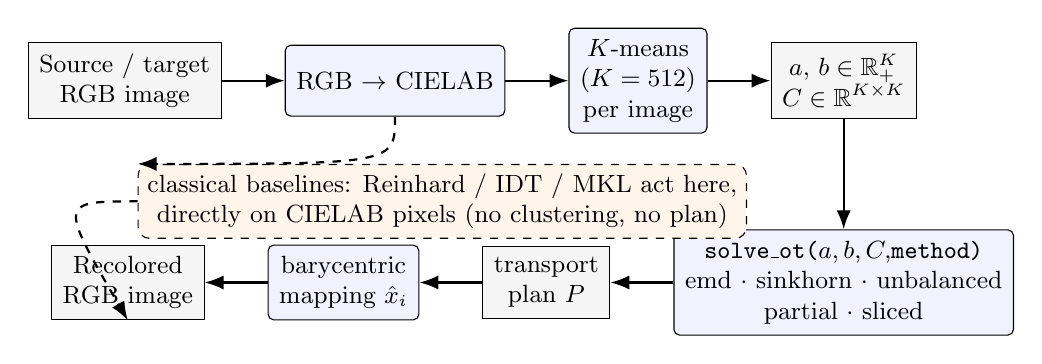
\begin{tikzpicture}[
    font=\small,
    box/.style={draw, rounded corners=2pt, align=center, minimum height=9mm,
                inner sep=4pt, fill=blue!5},
    data/.style={draw, align=center, minimum height=9mm, inner sep=4pt,
                 fill=gray!8},
    arr/.style={-{Latex[length=2.4mm]}, thick},
    node distance=6mm and 8mm,
  ]
  \node[data] (rgb) {Source / target\\ RGB image};
  \node[box, right=of rgb] (lab) {RGB $\to$ CIELAB};
  \node[box, right=of lab] (km) {$K$-means\\ ($K=512$)\\ per image};
  \node[data, right=of km] (abc) {$a,\,b \in \R_+^{K}$\\ $C \in \R^{K\times K}$};

  \node[box, below=14mm of abc] (solve) {\code{solve\_ot(}$a,b,C,$\code{method)}\\
        emd $\cdot$ sinkhorn $\cdot$ unbalanced\\ partial $\cdot$ sliced};
  \node[data, left=of solve] (plan) {transport\\ plan $P$};
  \node[box, left=of plan] (bary) {barycentric\\ mapping $\hat{x}_i$};
  \node[data, left=of bary] (out) {Recolored\\ RGB image};

  \draw[arr] (rgb) -- (lab);
  \draw[arr] (lab) -- (km);
  \draw[arr] (km) -- (abc);
  \draw[arr] (abc) -- (solve);
  \draw[arr] (solve) -- (plan);
  \draw[arr] (plan) -- (bary);
  \draw[arr] (bary) -- (out);

  \node[draw, dashed, rounded corners, fill=orange!8, align=center,
        below=6mm of lab, xshift=6mm] (base)
        {classical baselines: Reinhard / IDT / MKL act here,\\
         directly on CIELAB pixels (no clustering, no plan)};
  \draw[arr, dashed] (lab.south) .. controls +(0,-6mm) .. (base.north west);
  \draw[arr, dashed] (base.west) .. controls +(-10mm,0) .. (out.south);
\end{tikzpicture}
\caption{The unified color-transfer pipeline. OT methods follow the solid path;
classical baselines follow the dashed path.}
\label{fig:pipeline}
\end{figure}

\paragraph{Stage 1 -- color space.} Images are converted from sRGB to CIELAB,
which is approximately perceptually uniform, so that Euclidean distances are a
reasonable proxy for color difference.

\paragraph{Stage 2 -- quantization.} Each image is clustered independently with
$K$-means ($K = 512$, or fewer if the image has fewer pixels). Cluster $i$ of the
source has center $x_i$ and weight $a_i = (\text{\# pixels in cluster } i)/N$;
similarly $y_j, b_j$ for the target. This reduces the OT problem to
$512 \times 512$.

\paragraph{Stage 3 -- cost.} $C_{ij} = \lVert x_i - y_j \rVert_2^2$ between all
source/target center pairs (\code{ot.dist} with \code{metric="sqeuclidean"}).

\paragraph{Stage 4 -- solve.} \code{solve\_ot(a, b, C, method, \dots)} dispatches
to the POT routine for the chosen method and returns a plan
$P \in \R_+^{K \times K}$ (\cref{tab:dispatch}).

\begin{table}[t]
\centering
\caption{Dispatch table of \code{solve\_ot}. $\rho$ is \code{reg\_m}.}
\label{tab:dispatch}
\begin{tabular}{@{}llll@{}}
\toprule
\code{method} & POT routine & relaxation & key hyperparameters \\
\midrule
\code{emd}        & \code{ot.emd}                              & none (balanced) & --- \\
\code{sinkhorn}   & \code{ot.sinkhorn}                         & entropic        & $\varepsilon = 0.05\,\mathrm{median}(C)$ \\
\code{unbalanced} & \code{ot.unbalanced.sinkhorn\_unbalanced}  & KL marginals    & $\varepsilon,\ \rho$ \\
\code{partial}    & \code{ot.partial.partial\_wasserstein}     & mass $\le a,b$  & $m \in (0,1]$ \\
\code{sliced}     & mean of \code{ot.emd\_1d} over $L$ slices  & 1-D projections & $L = 100$ \\
\bottomrule
\end{tabular}
\end{table}

\paragraph{Stage 5 -- barycentric mapping.} Each source cluster $i$ is recolored
to the $P$-weighted average of the target centers,
\begin{equation}
  \label{eq:bary}
  \hat{x}_i \;=\; \frac{\sum_j P_{ij}\, y_j}{\sum_j P_{ij}},
\end{equation}
and every pixel adopts the new color of its cluster. For partial and unbalanced
OT the rows of $P$ do not sum to $a_i$; the undelivered mass is treated as
\emph{staying at the source color}:
\begin{equation}
  \label{eq:bary-keep}
  \hat{x}_i
  \;=\; \frac{\sum_j P_{ij}\, y_j \;+\; \bigl(a_i - \sum_j P_{ij}\bigr)\, x_i}
             {a_i},
\end{equation}
so a cluster that ships only $30\%$ of its mass ends up $70\%$ its original
color rather than fully recolored.

\subsection{Metrics}

We report a Pareto trade-off between two quantities plus a secondary check.

\begin{itemize}
  \item \textbf{$W_2$ color distance} (lower is better). Empirical $2$-Wasserstein
        distance between the \emph{result} colors and the \emph{target} colors in
        CIELAB: subsample $2000$ pixels from each, form the squared-Euclidean
        cost, and take $\sqrt{\code{ot.emd2}(\cdot)}$. Measures palette fidelity.
  \item \textbf{SSIM to source} (higher is better). Structural similarity between
        the result and the \emph{original source} image. Measures how much
        content / structure survived the recoloring.
  \item \textbf{Histogram intersection} (higher is better). $\sum \min(h_r, h_t)$
        over a $16^3$ RGB histogram; a coarse palette-overlap sanity check.
\end{itemize}

A method is good if it reaches \emph{low} $W_2$ (matches the target palette)
\emph{and} keeps \emph{high} SSIM (does not destroy the source). Balanced OT, we
will see, can only do the former.

\section{Experimental Setup}
\label{sec:setup}

\paragraph{Images.} Unless stated otherwise we use synthetic image pairs
generated with NumPy so the experiment is fully reproducible and the color
statistics are known exactly. Two scenarios:
\begin{itemize}
  \item \emph{Benchmark pair} (\cref{sec:res-bench}): a green ``foliage'' source
        with a brown trunk band, and a red ``sunset sky'' target with a bright
        sun disc and dark foreground.
  \item \emph{Mismatch pair} (\cref{sec:res-mismatch}): source $A$ is
        $\approx 70\%$ green / $30\%$ brown; target $B$ is $\approx 70\%$
        orange / $30\%$ blue. Green has no color neighbor in $B$.
\end{itemize}
Real photographs can be supplied on the command line instead.

\paragraph{Default hyperparameters.} $K = 512$ (benchmark) or $64$ (mismatch,
where the palette is nearly piecewise-constant); Sinkhorn / unbalanced
$\varepsilon = 0.05\,\mathrm{median}(C)$ on the raw cost, or $\varepsilon = 0.02$
on the cost normalized to $[0,1]$ in the mismatch sweep; partial $m = 0.7$
(benchmark); sliced $L = 100$ projections; $K$-means seed $= 0$.

\paragraph{Environment.} Python~3, POT~0.9.7, scikit-learn~1.9, scikit-image~0.26,
NumPy~2.5, Matplotlib. Timings are single-run wall-clock on CPU.

\section{Results}
\label{sec:results}

\subsection{Overall benchmark}
\label{sec:res-bench}

\Cref{tab:bench} reports all eight methods on the benchmark pair and
\cref{fig:pareto} plots the Pareto plane; \cref{fig:montage} shows the images.

\begin{table}[t]
\centering
\caption{Benchmark pair, $K = 512$. $W_2$: distance to target colors (lower
better). SSIM: similarity to source (higher better). Hist.: $16^3$ histogram
intersection (higher better).}
\label{tab:bench}
\begin{tabular}{@{}llrrrr@{}}
\toprule
method & type & $W_2\;\downarrow$ & SSIM $\uparrow$ & Hist.\ $\uparrow$ & time (s) \\
\midrule
\code{emd}        & OT (balanced)  & \textbf{4.41}  & 0.240 & 0.815 & 0.10 \\
\code{sinkhorn}   & OT (balanced)  & 16.37 & 0.302 & 0.254 & 0.02 \\
\code{unbalanced} & OT             & 45.51 & 0.248 & 0.132 & 0.03 \\
\code{partial}    & OT             & 61.38 & 0.358 & 0.570 & 0.13 \\
\code{sliced}     & OT             & 21.95 & 0.389 & 0.208 & 0.07 \\
\code{reinhard}   & baseline       & 27.17 & \textbf{0.519} & 0.033 & 0.02 \\
\code{idt}        & baseline       & 7.02  & 0.297 & \textbf{0.927} & 0.45 \\
\code{mkl}        & baseline       & 18.91 & 0.295 & 0.115 & 0.02 \\
\bottomrule
\end{tabular}
\end{table}

\begin{figure}[t]
\centering
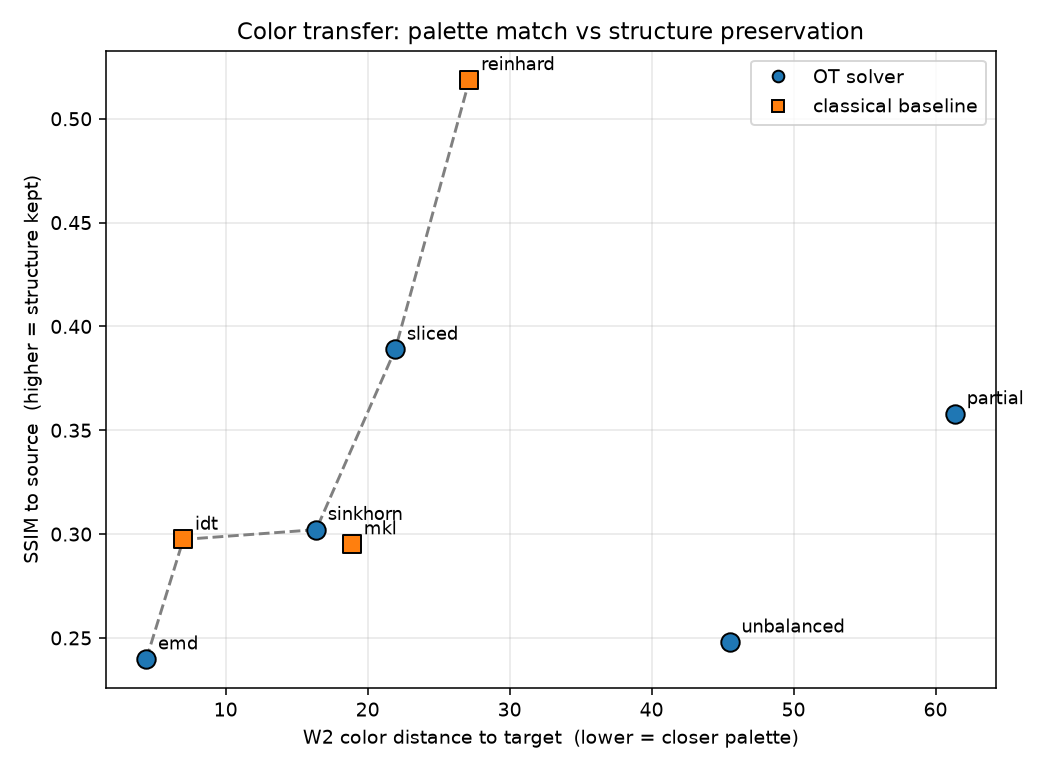
\includegraphics[width=0.86\linewidth]{pareto_plot.png}
\caption{Pareto plane for the benchmark pair. \code{emd} attains the best palette
match ($W_2 \approx 4$) but the worst structure score; the Pareto frontier is
formed by \code{emd}, \code{idt}, \code{sinkhorn}, \code{sliced}, and
\code{reinhard}.}
\label{fig:pareto}
\end{figure}

\begin{figure}[t]
\centering
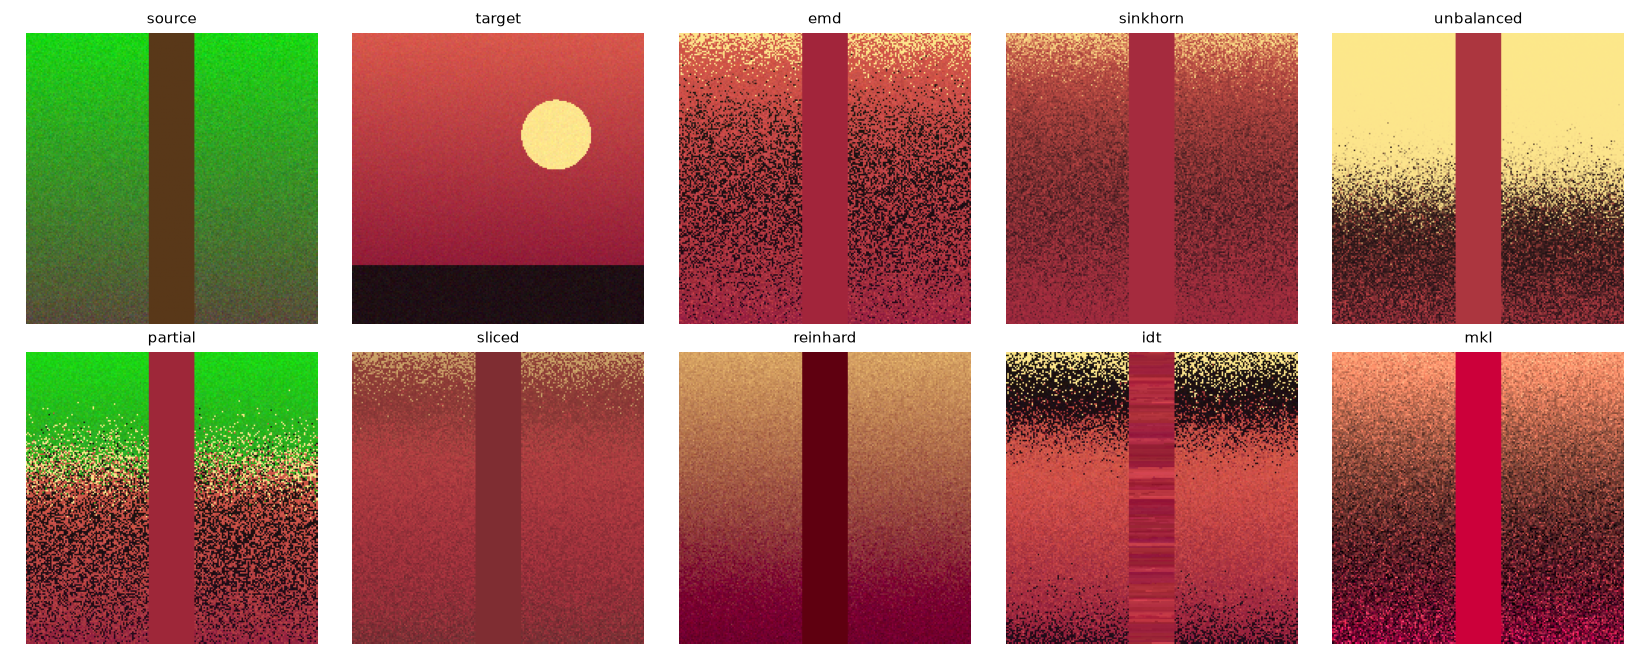
\includegraphics[width=\linewidth]{montage.png}
\caption{Benchmark pair: source, target, and the eight recolored results.
Cluster-based OT (\code{emd}, \code{sinkhorn}, \dots) produces salt-and-pepper
speckle because neighboring pixels belong to different clusters that are mapped
to different target colors; the global baselines (\code{reinhard}, \code{mkl})
are smooth continuous maps.}
\label{fig:montage}
\end{figure}

\paragraph{Observations.}
\begin{enumerate}
  \item \code{emd} minimizes $W_2$ (best palette match) but its SSIM ($0.240$) is
        essentially that of the target image itself: it reproduces the target
        palette by recoloring \emph{everything}.
  \item Among OT solvers, the relaxed variants (\code{partial}, \code{sliced})
        keep more structure (SSIM $0.36$--$0.39$) but at a much larger $W_2$ on
        this \emph{compatible} pair -- here there is no mismatch to exploit, so
        dropping mass only hurts palette fidelity.
  \item The global baselines \code{reinhard} and \code{mkl} preserve structure
        better than cluster-based OT because they are smooth per-pixel maps;
        cluster-based barycentric mapping introduces quantization speckle
        (\cref{fig:montage}).
  \item \code{idt} is the strongest baseline here (low $W_2$, high histogram
        intersection) as it explicitly matches the full 3-D distribution.
\end{enumerate}

\subsection{Distribution mismatch: the core experiment}
\label{sec:res-mismatch}

We now use the mismatch pair, where green has no counterpart in the target.
\Cref{tab:mismatch} and \cref{fig:mismatch} sweep EMD against unbalanced OT
(varying $\rho = \code{reg\_m} \in \{0.1, 1, 10\}$) and partial OT
(varying $m \in \{0.5, 0.7, 0.9\}$), with the cost normalized to $[0,1]$ so the
$\rho$ values span the useful range.

\begin{table}[t]
\centering
\caption{Mismatch pair, $K = 64$, cost normalized to $[0,1]$.}
\label{tab:mismatch}
\begin{tabular}{@{}lrr@{}}
\toprule
configuration & $W_2$ to target $\downarrow$ & SSIM to source $\uparrow$ \\
\midrule
source (identity)            & 92.37 & 1.000 \\
\code{EMD} (balanced)        & 12.43 & 0.538 \\
\code{unbalanced} $\rho=0.1$ & 87.45 & \textbf{0.815} \\
\code{unbalanced} $\rho=1$   & 32.13 & 0.583 \\
\code{unbalanced} $\rho=10$  & 10.86 & 0.556 \\
\code{partial} $m=0.5$       & 82.10 & 0.609 \\
\code{partial} $m=0.7$       & 73.54 & 0.585 \\
\code{partial} $m=0.9$       & 39.98 & 0.422 \\
\bottomrule
\end{tabular}
\end{table}

\begin{figure}[t]
\centering
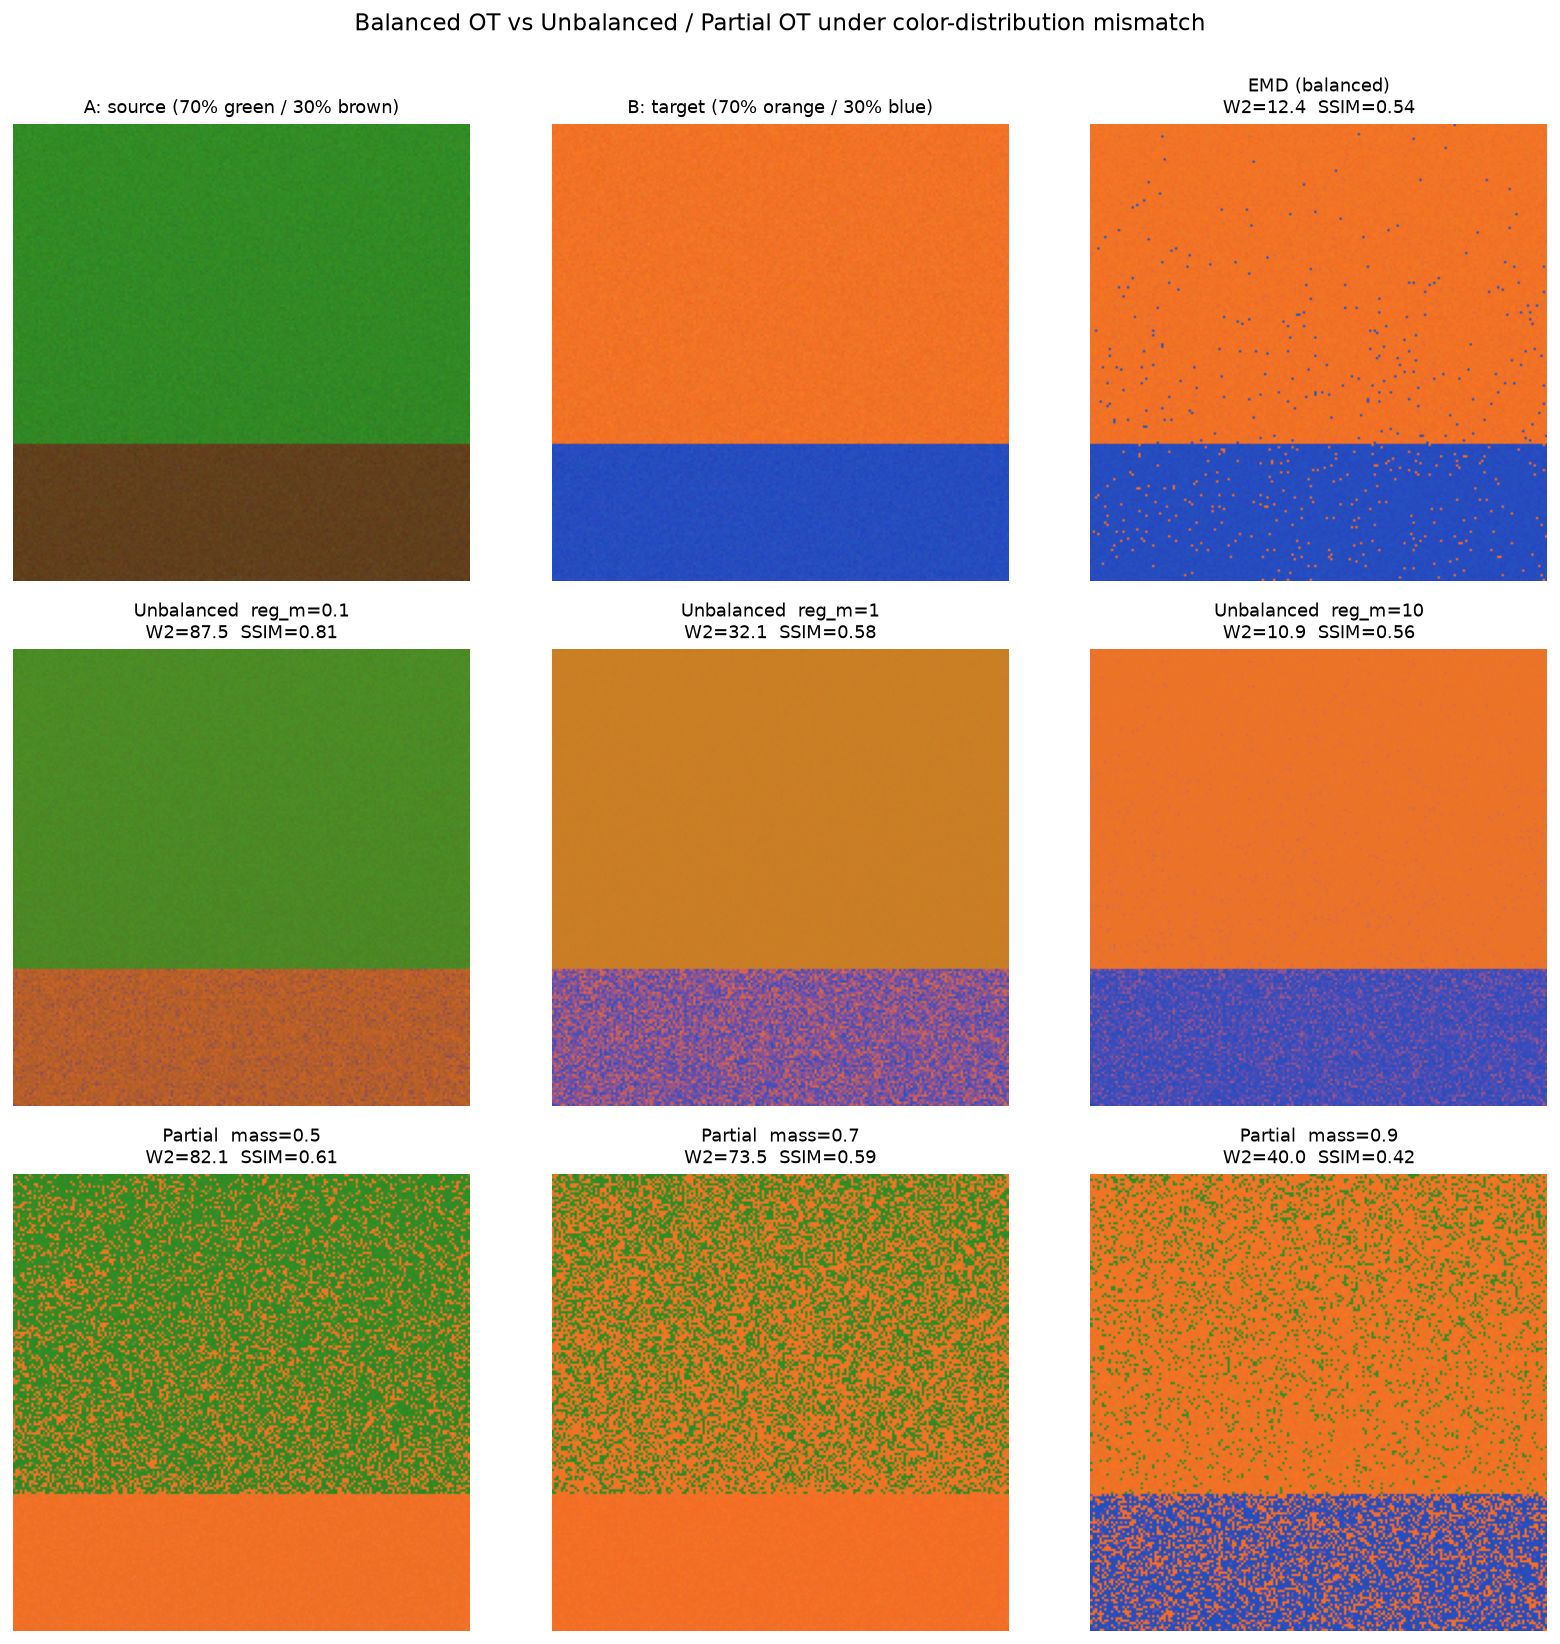
\includegraphics[width=\linewidth]{mismatch_comparison.png}
\caption{Mismatch pair. \textbf{Top row}: source $A$ ($70\%$ green / $30\%$
brown), target $B$ ($70\%$ orange / $30\%$ blue), and \code{EMD}. \textbf{Middle
row}: unbalanced OT, $\rho \in \{0.1, 1, 10\}$. \textbf{Bottom row}: partial OT,
$m \in \{0.5, 0.7, 0.9\}$. EMD recolors the green canopy fully to orange and the
brown soil fully to blue; unbalanced $\rho=0.1$ leaves the canopy green.}
\label{fig:mismatch}
\end{figure}

\paragraph{Observations.}
\begin{enumerate}
  \item \textbf{EMD forces implausible matches.} The green canopy becomes solid
        orange and the brown soil becomes solid blue -- the hard marginal
        constraint requires the plan to deliver exactly $30\%$ blue mass, and the
        only source mass available is green/brown.
  \item \textbf{Unbalanced OT recovers with small $\rho$.} At $\rho = 0.1$ the
        canopy stays green (SSIM $0.815$ vs.\ EMD's $0.538$); only the region
        with a plausible target shifts. As $\rho$ grows the result moves back
        toward EMD ($\rho = 10$: SSIM $0.556$, nearly identical to balanced).
  \item \textbf{Partial OT recovers by capping mass.} At $m = 0.5$ only the
        cheapest half of the mass is moved and the rest is kept; $m = 0.9$
        approaches balanced.
  \item Both knobs are monotone interpolators between ``identity'' and
        ``balanced OT''.
\end{enumerate}

\section{Discussion}
\label{sec:discussion}

\paragraph{Why balanced OT breaks.} The feasible set $U(a,b)$ in
\cref{eq:polytope} contains \emph{only} plans that move all source mass and
exactly reproduce the target marginal. When $\mathrm{supp}(a)$ and
$\mathrm{supp}(b)$ are far apart in color space -- a semantic mismatch -- every
$P \in U(a,b)$ has large cost and, worse, pairs colors that should be unrelated
(green $\to$ blue). The objective \cref{eq:kanto} has no term that rewards
``leaving a color alone''; it \emph{cannot} express that preference.

\paragraph{Unbalanced vs.\ partial.} Both introduce the missing option -- to not
transport some mass -- but through different knobs:
\begin{itemize}
  \item Unbalanced OT (\cref{eq:unbalanced}) softens the marginal constraint with
        a penalty of tunable strength $\rho$. It is smooth and symmetric
        (it can under- \emph{and} over-shoot a marginal), and $\rho$ lives in
        cost units, which makes it scale-dependent and less interpretable.
  \item Partial OT (\cref{eq:partial}) caps the transported \emph{mass fraction}
        $m$ directly. $m$ is a single, interpretable number in $[0,1]$, but the
        solver -- not the user -- decides \emph{which} mass to keep.
\end{itemize}

\paragraph{The cost: an extra hyperparameter.} Neither $\rho$ nor $m$ has a value
that is correct for every pair. \Cref{tab:mismatch} shows the SSIM/$W_2$
trade-off sliding continuously as the knob turns; the ``right'' setting depends
on how much of the source genuinely has no counterpart in the target, which is
exactly the unknown quantity. In practice this needs either domain knowledge or
a validation signal.

\paragraph{Limitations.}
\begin{itemize}
  \item Experiments use synthetic images; real photographs have smoother,
        higher-dimensional color manifolds.
  \item Cluster-based barycentric mapping (\cref{eq:bary}) causes spatial speckle
        (\cref{fig:montage}); a spatially-regularized OT
        (e.g.\ a Laplacian penalty on the map) or a larger $K$ with post-hoc
        smoothing would mitigate this.
  \item Our sliced-OT ``plan'' is an average of 1-D couplings, not a true
        transport map; a Monge-style 1-D transport composition would be more
        faithful.
  \item Metrics are global color statistics; they do not measure local
        color-consistency artifacts.
\end{itemize}

\section{Conclusion}
\label{sec:conclusion}

Balanced optimal transport is the natural formulation of color transfer only when
the two palettes are compatible. Its hard marginal constraints make it fail under
a semantic color-distribution mismatch: it recolors regions it should not touch,
trading almost all structural similarity for palette fidelity. Unbalanced OT and
partial OT both fix this by allowing mass to be left in place, and each reduces to
balanced OT in the appropriate limit ($\rho \to \infty$, $m \to 1$). The price is
one extra hyperparameter that interpolates the SSIM/$W_2$ trade-off and has no
universally correct value.

\paragraph{Future work.} Spatially-regularized / Laplacian OT to remove speckle;
automatic selection of $\rho$ or $m$ from a held-out signal; evaluation on a
real-photograph benchmark with mismatched semantics; a true transport map for
sliced OT.

\section*{Reproducibility}

\begin{verbatim}
pip install -r requirements.txt
python experiments/run_benchmark.py      # Table 1, Figures 2-3
python experiments/mismatch_demo.py      # Table 2, Figure 4
\end{verbatim}
Source modules: \code{color\_pipeline.py} (pipeline stages 1--3),
\code{solvers.py} (stage 4), \code{barycentric.py} (stage 5),
\code{baselines.py} (Reinhard / IDT / MKL), \code{metrics.py} (evaluation).

\begin{thebibliography}{9}

\bibitem{reinhard2001}
E.~Reinhard, M.~Ashikhmin, B.~Gooch, and P.~Shirley.
\newblock Color transfer between images.
\newblock \emph{IEEE Computer Graphics and Applications}, 21(5):34--41, 2001.

\bibitem{pitie2007idt}
F.~Piti\'e, A.~C. Kokaram, and R.~Dahyot.
\newblock Automated colour grading using colour distribution transfer.
\newblock \emph{Computer Vision and Image Understanding}, 107(1--2):123--137, 2007.

\bibitem{pitie2007mkl}
F.~Piti\'e and A.~Kokaram.
\newblock The linear Monge--Kantorovitch linear colour mapping for
  example-based colour transfer.
\newblock In \emph{4th European Conf.\ on Visual Media Production (CVMP)}, 2007.

\bibitem{cuturi2013}
M.~Cuturi.
\newblock Sinkhorn distances: Lightspeed computation of optimal transport.
\newblock In \emph{Advances in Neural Information Processing Systems (NeurIPS)}, 2013.

\bibitem{chizat2018}
L.~Chizat, G.~Peyr\'e, B.~Schmitzer, and F.-X. Vialard.
\newblock Scaling algorithms for unbalanced optimal transport problems.
\newblock \emph{Mathematics of Computation}, 87(314):2563--2609, 2018.

\bibitem{chapel2020}
L.~Chapel, M.~Z. Alaya, and G.~Gasso.
\newblock Partial optimal transport with applications on positive-unlabeled
  learning.
\newblock In \emph{Advances in Neural Information Processing Systems (NeurIPS)}, 2020.

\bibitem{bonneel2015}
N.~Bonneel, J.~Rabin, G.~Peyr\'e, and H.~Pfister.
\newblock Sliced and Radon Wasserstein barycenters of measures.
\newblock \emph{Journal of Mathematical Imaging and Vision}, 51(1):22--45, 2015.

\bibitem{ferradans2014}
S.~Ferradans, N.~Papadakis, G.~Peyr\'e, and J.-F. Aujol.
\newblock Regularized discrete optimal transport.
\newblock \emph{SIAM Journal on Imaging Sciences}, 7(3):1853--1882, 2014.

\bibitem{pot2021}
R.~Flamary et al.
\newblock POT: Python Optimal Transport.
\newblock \emph{Journal of Machine Learning Research}, 22(78):1--8, 2021.

\end{thebibliography}

\end{document}
